\documentclass[]{article}
\usepackage{lmodern}
\usepackage{amssymb,amsmath}
\usepackage{ifxetex,ifluatex}
\usepackage{fixltx2e} % provides \textsubscript
\ifnum 0\ifxetex 1\fi\ifluatex 1\fi=0 % if pdftex
  \usepackage[T1]{fontenc}
  \usepackage[utf8]{inputenc}
\else % if luatex or xelatex
  \ifxetex
    \usepackage{mathspec}
  \else
    \usepackage{fontspec}
  \fi
  \defaultfontfeatures{Ligatures=TeX,Scale=MatchLowercase}
\fi
% use upquote if available, for straight quotes in verbatim environments
\IfFileExists{upquote.sty}{\usepackage{upquote}}{}
% use microtype if available
\IfFileExists{microtype.sty}{%
\usepackage{microtype}
\UseMicrotypeSet[protrusion]{basicmath} % disable protrusion for tt fonts
}{}
\usepackage[margin=1in]{geometry}
\usepackage{hyperref}
\hypersetup{unicode=true,
            pdftitle={title},
            pdfborder={0 0 0},
            breaklinks=true}
\urlstyle{same}  % don't use monospace font for urls
\usepackage{color}
\usepackage{fancyvrb}
\newcommand{\VerbBar}{|}
\newcommand{\VERB}{\Verb[commandchars=\\\{\}]}
\DefineVerbatimEnvironment{Highlighting}{Verbatim}{commandchars=\\\{\}}
% Add ',fontsize=\small' for more characters per line
\usepackage{framed}
\definecolor{shadecolor}{RGB}{248,248,248}
\newenvironment{Shaded}{\begin{snugshade}}{\end{snugshade}}
\newcommand{\KeywordTok}[1]{\textcolor[rgb]{0.13,0.29,0.53}{\textbf{#1}}}
\newcommand{\DataTypeTok}[1]{\textcolor[rgb]{0.13,0.29,0.53}{#1}}
\newcommand{\DecValTok}[1]{\textcolor[rgb]{0.00,0.00,0.81}{#1}}
\newcommand{\BaseNTok}[1]{\textcolor[rgb]{0.00,0.00,0.81}{#1}}
\newcommand{\FloatTok}[1]{\textcolor[rgb]{0.00,0.00,0.81}{#1}}
\newcommand{\ConstantTok}[1]{\textcolor[rgb]{0.00,0.00,0.00}{#1}}
\newcommand{\CharTok}[1]{\textcolor[rgb]{0.31,0.60,0.02}{#1}}
\newcommand{\SpecialCharTok}[1]{\textcolor[rgb]{0.00,0.00,0.00}{#1}}
\newcommand{\StringTok}[1]{\textcolor[rgb]{0.31,0.60,0.02}{#1}}
\newcommand{\VerbatimStringTok}[1]{\textcolor[rgb]{0.31,0.60,0.02}{#1}}
\newcommand{\SpecialStringTok}[1]{\textcolor[rgb]{0.31,0.60,0.02}{#1}}
\newcommand{\ImportTok}[1]{#1}
\newcommand{\CommentTok}[1]{\textcolor[rgb]{0.56,0.35,0.01}{\textit{#1}}}
\newcommand{\DocumentationTok}[1]{\textcolor[rgb]{0.56,0.35,0.01}{\textbf{\textit{#1}}}}
\newcommand{\AnnotationTok}[1]{\textcolor[rgb]{0.56,0.35,0.01}{\textbf{\textit{#1}}}}
\newcommand{\CommentVarTok}[1]{\textcolor[rgb]{0.56,0.35,0.01}{\textbf{\textit{#1}}}}
\newcommand{\OtherTok}[1]{\textcolor[rgb]{0.56,0.35,0.01}{#1}}
\newcommand{\FunctionTok}[1]{\textcolor[rgb]{0.00,0.00,0.00}{#1}}
\newcommand{\VariableTok}[1]{\textcolor[rgb]{0.00,0.00,0.00}{#1}}
\newcommand{\ControlFlowTok}[1]{\textcolor[rgb]{0.13,0.29,0.53}{\textbf{#1}}}
\newcommand{\OperatorTok}[1]{\textcolor[rgb]{0.81,0.36,0.00}{\textbf{#1}}}
\newcommand{\BuiltInTok}[1]{#1}
\newcommand{\ExtensionTok}[1]{#1}
\newcommand{\PreprocessorTok}[1]{\textcolor[rgb]{0.56,0.35,0.01}{\textit{#1}}}
\newcommand{\AttributeTok}[1]{\textcolor[rgb]{0.77,0.63,0.00}{#1}}
\newcommand{\RegionMarkerTok}[1]{#1}
\newcommand{\InformationTok}[1]{\textcolor[rgb]{0.56,0.35,0.01}{\textbf{\textit{#1}}}}
\newcommand{\WarningTok}[1]{\textcolor[rgb]{0.56,0.35,0.01}{\textbf{\textit{#1}}}}
\newcommand{\AlertTok}[1]{\textcolor[rgb]{0.94,0.16,0.16}{#1}}
\newcommand{\ErrorTok}[1]{\textcolor[rgb]{0.64,0.00,0.00}{\textbf{#1}}}
\newcommand{\NormalTok}[1]{#1}
\usepackage{graphicx,grffile}
\makeatletter
\def\maxwidth{\ifdim\Gin@nat@width>\linewidth\linewidth\else\Gin@nat@width\fi}
\def\maxheight{\ifdim\Gin@nat@height>\textheight\textheight\else\Gin@nat@height\fi}
\makeatother
% Scale images if necessary, so that they will not overflow the page
% margins by default, and it is still possible to overwrite the defaults
% using explicit options in \includegraphics[width, height, ...]{}
\setkeys{Gin}{width=\maxwidth,height=\maxheight,keepaspectratio}
\IfFileExists{parskip.sty}{%
\usepackage{parskip}
}{% else
\setlength{\parindent}{0pt}
\setlength{\parskip}{6pt plus 2pt minus 1pt}
}
\setlength{\emergencystretch}{3em}  % prevent overfull lines
\providecommand{\tightlist}{%
  \setlength{\itemsep}{0pt}\setlength{\parskip}{0pt}}
\setcounter{secnumdepth}{0}
% Redefines (sub)paragraphs to behave more like sections
\ifx\paragraph\undefined\else
\let\oldparagraph\paragraph
\renewcommand{\paragraph}[1]{\oldparagraph{#1}\mbox{}}
\fi
\ifx\subparagraph\undefined\else
\let\oldsubparagraph\subparagraph
\renewcommand{\subparagraph}[1]{\oldsubparagraph{#1}\mbox{}}
\fi

%%% Use protect on footnotes to avoid problems with footnotes in titles
\let\rmarkdownfootnote\footnote%
\def\footnote{\protect\rmarkdownfootnote}

%%% Change title format to be more compact
\usepackage{titling}

% Create subtitle command for use in maketitle
\providecommand{\subtitle}[1]{
  \posttitle{
    \begin{center}\large#1\end{center}
    }
}

\setlength{\droptitle}{-2em}

  \title{title}
    \pretitle{\vspace{\droptitle}\centering\huge}
  \posttitle{\par}
    \author{}
    \preauthor{}\postauthor{}
      \predate{\centering\large\emph}
  \postdate{\par}
    \date{2019-05-03 22:24:25}


\begin{document}
\maketitle

{
\setcounter{tocdepth}{3}
\tableofcontents
}
\section{Working Environment}\label{working-environment}

\subsection{Working With Bash and Git}\label{working-with-bash-and-git}

\subsubsection{Useful Commands}\label{useful-commands}

\begin{Shaded}
\begin{Highlighting}[]
\FunctionTok{login}\NormalTok{     # prompts for username and then password to log in}
\FunctionTok{man}\NormalTok{       # man (command) }\ExtensionTok{returns}\NormalTok{ documentation a command}
\end{Highlighting}
\end{Shaded}

\subsection{Directory Commands}

\begin{Shaded}
\begin{Highlighting}[]
\BuiltInTok{pwd}\NormalTok{       # print working directory}
\BuiltInTok{cd}\NormalTok{        # changes directory to home}
\BuiltInTok{cd} \DataTypeTok{\textbackslash{} }\NormalTok{     # changes directory to (/path)}
\BuiltInTok{cd}\NormalTok{ ..     # moves up one folder in the directory}
\FunctionTok{ls}\NormalTok{ -al    # lists contencts of directory, -a includes hidden items, -l includes details}
\end{Highlighting}
\end{Shaded}

~is also used to include the space characters in a file name,
e.g.~Google~Drive.

\subsection{File Operations}

\begin{Shaded}
\begin{Highlighting}[]
\FunctionTok{mkdir}\NormalTok{    # make a new directory}
\FunctionTok{touch}\NormalTok{    # create a file}
\ExtensionTok{open}\NormalTok{     # open a file}
\FunctionTok{mv}\NormalTok{       # move (file) }\KeywordTok{(}\ExtensionTok{to}\KeywordTok{)}\NormalTok{, }\ExtensionTok{can}\NormalTok{ also be used to rename a file}
\FunctionTok{cp}\NormalTok{       # copy (file) }\KeywordTok{(}\ExtensionTok{to}\KeywordTok{)} 
\FunctionTok{rm}\NormalTok{       # delete a file}
\end{Highlighting}
\end{Shaded}

\subsection{Other Utilities}

\begin{Shaded}
\begin{Highlighting}[]
\BuiltInTok{echo}\NormalTok{    # print commands screen}
\FunctionTok{date}\NormalTok{    # print date}
\FunctionTok{cal}\NormalTok{     # print calendar (year)}
\end{Highlighting}
\end{Shaded}

\subsection{Creating and Sourcing Custom Commands}

The sections below are based on information in
\href{https://medium.com/devnetwork/how-to-create-your-own-custom-terminal-commands-c5008782a78e}{\color{blue} this Medium blog post}
and
\href{https://stackoverflow.com/questions/19662713/where-do-i-find-the-bashrc-file-on-mac}{\color{blue}this StackOverflow post}.

\subsubsection{Creating Commands}

Use the alias command to map an execution of bash commands to a single
command. For example, this will create a command `hi' where the Luca
voice slowly says `hello world';

\begin{Shaded}
\begin{Highlighting}[]
\BuiltInTok{alias}\NormalTok{ hi=}\StringTok{"say -v Luca  -r 100 'hello world'"}
\ExtensionTok{hi} \CommentTok{# test this alias}
\end{Highlighting}
\end{Shaded}

Functions can be created with the following syntax;

\begin{Shaded}
\begin{Highlighting}[]
\KeywordTok{function}\FunctionTok{ function_name()} \KeywordTok{\{}
 \OperatorTok{<}\ExtensionTok{args}\OperatorTok{>} 
\KeywordTok{\}}
\end{Highlighting}
\end{Shaded}

Inputs are denoted with \$1, \$2, \ldots{} . For example, when called
from the terminal, this function will print `Your Input Was:' followed
by the first argument it receives;

\begin{Shaded}
\begin{Highlighting}[]
\KeywordTok{function}\FunctionTok{ print_my_input()} \KeywordTok{\{}
 \BuiltInTok{echo} \StringTok{'Your Input Was:'} \VariableTok{$1} 
\KeywordTok{\}}
\end{Highlighting}
\end{Shaded}

To create a file where custom commands are defined, navigate to the home
directory, create, and open the file that will hold function
definitions;

\begin{Shaded}
\begin{Highlighting}[]
\BuiltInTok{cd} 
\FunctionTok{touch}\NormalTok{ .custom_commands}
\ExtensionTok{open}\NormalTok{ .custom_commands}
\end{Highlighting}
\end{Shaded}

Define commands you wish to use in future Terminal sessions in the
.custom\_commands file. The next section describes how to source this
file automatically when a Terminal session is initialized.

\subsubsection{Sourcing Files During Terminal Initialization}

Bash sources a run control file (\textasciitilde{}/.bashrc) at
initialization. Check if this file exists in the home directory with;

\begin{Shaded}
\begin{Highlighting}[]
\BuiltInTok{cd}
\FunctionTok{ls}\NormalTok{ -a}
\end{Highlighting}
\end{Shaded}

If there is no .bashrc file listed, then first open the .bash\_profile
file in a text editor and add the following;

\begin{Shaded}
\begin{Highlighting}[]
\KeywordTok{if}\BuiltInTok{ [} \OtherTok{-f}\NormalTok{ ~/.bashrc}\BuiltInTok{ ]}\NormalTok{; }\KeywordTok{then}
    \BuiltInTok{.} \ExtensionTok{~/.bashrc}
\KeywordTok{fi}
\end{Highlighting}
\end{Shaded}

Then create and open a .bashrc file in the home directory with;

\begin{Shaded}
\begin{Highlighting}[]
\BuiltInTok{cd}
\FunctionTok{touch}\NormalTok{ .bashrc}
\ExtensionTok{open}\NormalTok{ .bashrc}
\end{Highlighting}
\end{Shaded}

In a text editor add the following lines to the .bashrc file;

\begin{Shaded}
\begin{Highlighting}[]
\CommentTok{# Source global definitions}
\KeywordTok{if}\BuiltInTok{ [} \OtherTok{-f}\NormalTok{ /etc/bashrc}\BuiltInTok{ ]}\NormalTok{; }\KeywordTok{then}
    \BuiltInTok{.} \ExtensionTok{/etc/bashrc}
\KeywordTok{fi}

\CommentTok{# source file with function definitions}
\BuiltInTok{source}\NormalTok{ ~/.custom_commands}
\end{Highlighting}
\end{Shaded}

This last line will source the .custom\_commands file described at the
end of the previous section, thereby defining any aliases or functions
in the .custom\_commands file whenever a Terminal session is
initialized.

\subsection{Scheduling Bash Functions With Crontab}

Some basic crontab commands;

\begin{Shaded}
\begin{Highlighting}[]
\ExtensionTok{crontab}\NormalTok{ -l }\CommentTok{# lists crontab jobs}
\ExtensionTok{crontab}\NormalTok{ -r }\CommentTok{# removes all crontab jobs}
\ExtensionTok{crontab}\NormalTok{ -e }\CommentTok{# edits list of crontab jobs}
\end{Highlighting}
\end{Shaded}

The crontab -e command is somewhat hard to navigate, the following code
is an easier way to create crontab jobs from ther terminal;

\begin{Shaded}
\begin{Highlighting}[]
\ExtensionTok{crontab}\NormalTok{ -l }\KeywordTok{|} \KeywordTok{\{} \FunctionTok{cat}\KeywordTok{;} \BuiltInTok{echo} \StringTok{"* * * * * some entry"}\KeywordTok{;} \KeywordTok{\}} \KeywordTok{|} \ExtensionTok{crontab}\NormalTok{ -}

\CommentTok{# format for string argument for crontab;}
\ExtensionTok{*}\NormalTok{ * * * * }\StringTok{"some entry"}
\ExtensionTok{-}\NormalTok{ - - - -}
\KeywordTok{|} \KeywordTok{|} \KeywordTok{|} \KeywordTok{|} \KeywordTok{|}
\KeywordTok{|} \KeywordTok{|} \KeywordTok{|} \KeywordTok{|} \ExtensionTok{-----}\NormalTok{ Day of week (0 - 7) }\KeywordTok{(}\VariableTok{Sunday=}\NormalTok{0 }\ExtensionTok{or}\NormalTok{ 7}\KeywordTok{)}
\KeywordTok{|} \KeywordTok{|} \KeywordTok{|} \ExtensionTok{-------}\NormalTok{ Month (1 - 12)}
\KeywordTok{|} \KeywordTok{|} \ExtensionTok{---------}\NormalTok{ Day of month (1 - 31)}
\KeywordTok{|} \ExtensionTok{-----------}\NormalTok{ Hour (0 - 23)}
\ExtensionTok{-------------}\NormalTok{ Minute (0 - 59)}
\end{Highlighting}
\end{Shaded}

I simplify this farther in a custom function called `schedule' that I
define in \ref{sec: schedule}.

To execute functions from a user, the user must be specified in
/etc/cron.allow -- however, this file can only be edited by a superuser.
To create and edit this file, use;

\begin{Shaded}
\begin{Highlighting}[]
\BuiltInTok{cd}\NormalTok{ /etc}
\FunctionTok{sudo}\NormalTok{ touch cron.allow}
\FunctionTok{sudo}\NormalTok{ nano cron.allow}
\end{Highlighting}
\end{Shaded}

nano opens a text editor in ther terminal, and that can be used to edit
and save changes to cron.allow.

More information on crontab
\href{https://www.computerhope.com/unix/ucrontab.htm}{\color{blue} here}.

\section{Git and GitHub}

\subsection{Setup}

\begin{Shaded}
\begin{Highlighting}[]
\CommentTok{# create user name and email for tagging contributions later}
\FunctionTok{git}\NormalTok{ config --global user.name }\StringTok{"Mac Strelioff"}   
\FunctionTok{git}\NormalTok{ config --global user.email }\StringTok{"mstrelio@uci.edu"} 
\end{Highlighting}
\end{Shaded}

Connecting to Git can be done through a username/password or through SSH
verification.

\subsubsection{Username/Password}

This didn't work for ubdates scheduled through crontab.

\subsubsection{SSH}

First,
\href{https://help.github.com/articles/checking-for-existing-ssh-keys/}{\color{blue}check for SSH keys with};

\begin{Shaded}
\begin{Highlighting}[]
\BuiltInTok{cd}\NormalTok{ ~/.ssh  # navigate to user/.ssh folder}
\FunctionTok{ls}\NormalTok{ -a      # list all files}
\end{Highlighting}
\end{Shaded}

A public SSH key is in id\_rsa.pub, which can be opened in a text
editor.

If no id\_rsa file exists, or if you wish to create a new SSH key, you
can use the following command to generate a new SSH key;

\begin{Shaded}
\begin{Highlighting}[]
\FunctionTok{ssh-keygen}\NormalTok{ -t rsa -b 4096 -C }\StringTok{"your_email@example.com"} \CommentTok{# run this if id_rsa file does not exist}
\end{Highlighting}
\end{Shaded}

This will prompt you for the file location where the SSH key should be
saved -- id\_rsa is the default file.

From here, follow the steps
\href{https://help.github.com/articles/generating-a-new-ssh-key-and-adding-it-to-the-ssh-agent/}{\color{blue}to add an SSH key},
summarized below.

First, create a config file for the SSH agent with;

\begin{Shaded}
\begin{Highlighting}[]
\FunctionTok{touch}\NormalTok{ ~/.ssh/config}
\end{Highlighting}
\end{Shaded}

Open the config file in a text editor and add the the following
commands;

\begin{Shaded}
\begin{Highlighting}[]
\ExtensionTok{Host}\NormalTok{ *}
 \ExtensionTok{AddKeysToAgent}\NormalTok{ yes}
 \ExtensionTok{UseKeychain}\NormalTok{ yes}
 \ExtensionTok{IdentityFile}\NormalTok{ ~/.ssh/id_rsa}
\end{Highlighting}
\end{Shaded}

Next, from Terminal, add the key from the file (e.g.~id\_rsa) to the ssh
agent with;

\begin{Shaded}
\begin{Highlighting}[]
\FunctionTok{ssh-add}\NormalTok{ -K ~/.ssh/id_rsa}
\end{Highlighting}
\end{Shaded}

Finally,
\href{https://help.github.com/articles/adding-a-new-ssh-key-to-your-github-account/}{\color{blue}add the ssh key to the GitHub account}.

And
\href{https://help.github.com/articles/testing-your-ssh-connection/}{\color{blue}test the connection}
with;

\begin{Shaded}
\begin{Highlighting}[]
\FunctionTok{ssh}\NormalTok{ -T git@github.com}
\end{Highlighting}
\end{Shaded}

\subsection{Working From a Repository}

Create a repository through GitHub's user interface (log in and select
`new repository').

Then create a directory on a local computer, possibly using bash
commands; mkdir and cd.

The simplest way is to clone the repo from GitHub with;

\begin{Shaded}
\begin{Highlighting}[]
\FunctionTok{git}\NormalTok{ clone (url)     # }\ExtensionTok{this}\NormalTok{ will clone from the url to the current directory}
\end{Highlighting}
\end{Shaded}

Another way, from inside the directory that is to be the local repo,
issue these commands;

\begin{Shaded}
\begin{Highlighting}[]
\FunctionTok{git}\NormalTok{ init   # initialize a repo}
\FunctionTok{git}\NormalTok{ remote add origin (url or SSH address) }\CommentTok{# point local repo to remote repo}
\end{Highlighting}
\end{Shaded}

\subsection{Switching between SSH and HTTPS Access}\label{sec:SwitchingHTTPStoSSH}

In both examples below, replace `USERNAME/REPOSITORY' with the
appropriate values. From within the local repo folder,

Change from HTTPS to SSH with;

\begin{Shaded}
\begin{Highlighting}[]
\FunctionTok{git}\NormalTok{ remote set-url origin git@github.com:USERNAME/REPOSITORY.git}
\FunctionTok{git}\NormalTok{ remote -v }\CommentTok{# list fetch and push destinations, should start with git@github.com}
\end{Highlighting}
\end{Shaded}

Change from SSH to HTTPS with;

\begin{Shaded}
\begin{Highlighting}[]
\FunctionTok{git}\NormalTok{ remote set-url origin https://github.com/USERNAME/REPOSITORY.git}
\FunctionTok{git}\NormalTok{ remote -v }\CommentTok{# list fetch and push destinations, should start with https://github.com/}
\end{Highlighting}
\end{Shaded}

\href{https://help.github.com/articles/changing-a-remote-s-url/}{\color{blue}More detailed guide here.}

Other methods for addressing `Device not configured' errors
\href{https://stackoverflow.com/questions/40274484/fatal-could-not-read-username-for-https-github-com-device-not-configured}{\color{blue}here}.

\subsection{Repository Maintanence And Collaboration}

\begin{Shaded}
\begin{Highlighting}[]
\CommentTok{# download.file("https://i.stack.imgur.com/nWYnQ.png",'y.jpg', mode = 'wb')}
\NormalTok{jj <-}\StringTok{ }\KeywordTok{readPNG}\NormalTok{(}\StringTok{"y.jpg"}\NormalTok{,}\DataTypeTok{native=}\OtherTok{TRUE}\NormalTok{)}
\KeywordTok{plot}\NormalTok{(}\DecValTok{0}\OperatorTok{:}\DecValTok{1}\NormalTok{,}\DecValTok{0}\OperatorTok{:}\DecValTok{1}\NormalTok{,}\DataTypeTok{type=}\StringTok{"n"}\NormalTok{,}\DataTypeTok{ann=}\OtherTok{FALSE}\NormalTok{,}\DataTypeTok{axes=}\OtherTok{FALSE}\NormalTok{)}
\KeywordTok{rasterImage}\NormalTok{(jj,}\DecValTok{0}\NormalTok{,}\DecValTok{0}\NormalTok{,}\DecValTok{1}\NormalTok{,}\DecValTok{1}\NormalTok{)}
\end{Highlighting}
\end{Shaded}

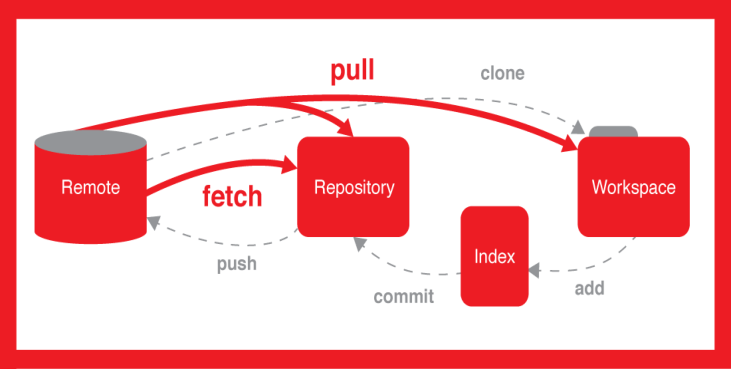
\includegraphics{Data-Science-Handbook_files/figure-latex/unnamed-chunk-27-1.pdf}

Useful commands;

\begin{Shaded}
\begin{Highlighting}[]
\FunctionTok{git}\NormalTok{ pull    # adds files from the configured remote repo to your local repo and workspace}
\FunctionTok{git}\NormalTok{ add .   # adds all new files to be tracked}
\FunctionTok{git}\NormalTok{ add -u  # updates all files}
\FunctionTok{git}\NormalTok{ add -A  # does both }\StringTok{'.'}\NormalTok{ and }\StringTok{'-u'}
\FunctionTok{git}\NormalTok{ commit -m }\StringTok{"message"} \CommentTok{# saves changes local repo}
\FunctionTok{git}\NormalTok{ push    # updates repo on GitHub}
\end{Highlighting}
\end{Shaded}

Collaborators can all access the GitHub repo through push/pull commands.
In collaborative settings you might need to pull, so that your
repository is current, before pushing changes from the local repository
to the remote repository on GitHub.

\subsection{Versioning}

\subsubsection{Branching}

\begin{Shaded}
\begin{Highlighting}[]
\FunctionTok{git}\NormalTok{ branch   # prints the current branch}
\FunctionTok{git}\NormalTok{ checkout -b branchname }\CommentTok{# creates new branch named branchname}
\FunctionTok{git}\NormalTok{ checkout master }\CommentTok{# changes back to master branch}
\end{Highlighting}
\end{Shaded}

\subsubsection{Merging}

TODO: add details on merging, and commit in terms of versioning

\subsection{Useful Custom Aliases and Functions}

\subsubsection{gitup: combines add, commit, and push into one command.}

\begin{Shaded}
\begin{Highlighting}[]
\BuiltInTok{alias}\NormalTok{ gitup=}\StringTok{"git add -A; git commit -m 'auto'; git push"}
\end{Highlighting}
\end{Shaded}

\subsubsection{gitupall: updates all git repos in my git folder}

\begin{Shaded}
\begin{Highlighting}[]
\KeywordTok{function}\FunctionTok{ gitupall}\KeywordTok{\{}
\KeywordTok{for} \ExtensionTok{filename}\NormalTok{ in /Users/mac/git/*}\KeywordTok{;} \KeywordTok{do}
\BuiltInTok{echo} \StringTok{"**************************updating }\VariableTok{$filename}\StringTok{"}
\BuiltInTok{cd} \StringTok{"}\VariableTok{$filename}\StringTok{"}\KeywordTok{;} 
\ExtensionTok{gitup}
\BuiltInTok{cd}\NormalTok{ ..}
\KeywordTok{done}
\KeywordTok{\}}
\end{Highlighting}
\end{Shaded}

\subsubsection{schedule: schedules a command to be executed periodically}\label{sec: schedule}

\begin{Shaded}
\begin{Highlighting}[]
\KeywordTok{function}\FunctionTok{ schedule()}\KeywordTok{\{}
\ExtensionTok{crontab}\NormalTok{ -l }\KeywordTok{|} \KeywordTok{\{} \FunctionTok{cat}\KeywordTok{;} \BuiltInTok{echo} \StringTok{"}\VariableTok{$1}\StringTok{"}\KeywordTok{;} \KeywordTok{\}} \KeywordTok{|} \ExtensionTok{crontab}\NormalTok{ -}
\KeywordTok{\}}

\CommentTok{# format for string argument for crontab;}
\ExtensionTok{*}\NormalTok{ * * * * }\StringTok{"command to be executed"}
\ExtensionTok{-}\NormalTok{ - - - -}
\KeywordTok{|} \KeywordTok{|} \KeywordTok{|} \KeywordTok{|} \KeywordTok{|}
\KeywordTok{|} \KeywordTok{|} \KeywordTok{|} \KeywordTok{|} \ExtensionTok{-----}\NormalTok{ Day of week (0 - 7) }\KeywordTok{(}\VariableTok{Sunday=}\NormalTok{0 }\ExtensionTok{or}\NormalTok{ 7}\KeywordTok{)}
\KeywordTok{|} \KeywordTok{|} \KeywordTok{|} \ExtensionTok{-------}\NormalTok{ Month (1 - 12)}
\KeywordTok{|} \KeywordTok{|} \ExtensionTok{---------}\NormalTok{ Day of month (1 - 31)}
\KeywordTok{|} \ExtensionTok{-----------}\NormalTok{ Hour (0 - 23)}
\ExtensionTok{-------------}\NormalTok{ Minute (0 - 59)}
\end{Highlighting}
\end{Shaded}

Example use;

\begin{Shaded}
\begin{Highlighting}[]
\CommentTok{# e.g. use: schedule updating of all repos each hour}
\ExtensionTok{schedule} \StringTok{"0 0-23 * * * gitupall"}
\ExtensionTok{crontab}\NormalTok{ -l }\CommentTok{# lists crontab jobs after schedule call}
\end{Highlighting}
\end{Shaded}

\subsubsection{cronrm: removes a scheduled command}

\begin{Shaded}
\begin{Highlighting}[]

\ExtensionTok{TODO}
\end{Highlighting}
\end{Shaded}

\section{Open Science Framework}

\subsection{Advantages of OSF}

OSF has no storage limits. OSF is also widely used by the behavioral
research community, and may be better apt for storing experimental data.

Maybe I'll delineate projects by data -\textgreater{} OSF, no data
-\textgreater{} Git.

\subsection{osfr R Package}

See
\href{https://centerforopenscience.github.io/osfr/}{\color{blue}R interface with OSF}.

\subsection{Authentication}

Personal acceess tokens can be created by logging in to OSF and
navigating to
\href{https://osf.io/settings/tokens/}{\color{blue}https://osf.io/settings/tokens/}

When creating a token, you will have the option to enable various
privilages or scopes. Give this token a limited scope, as it is easy for
anyone with access to R on your computer to reveal the token through the
last step presented here.

Once a token is created, add it to the home directory in a file called
`.Renviron' with the following terminal commands;

\begin{Shaded}
\begin{Highlighting}[]
\BuiltInTok{cd} \CommentTok{# navigate to home directory}
\FunctionTok{touch}\NormalTok{ .Renviron }\CommentTok{# create .Renviron file}
\ExtensionTok{open}\NormalTok{ .Renviron }\CommentTok{# open this file in a text editor}
\end{Highlighting}
\end{Shaded}

In a text editor, add the following line in the .Renviron file;

\begin{Shaded}
\begin{Highlighting}[]
\VariableTok{OSF_PAT=} \ExtensionTok{YOUR}\NormalTok{ PERSONAL ACCESS TOKEN}
\end{Highlighting}
\end{Shaded}

Replace YOUR PERSONAL ACCESS TOKEN with the token from OSF, and save the
.Renviron file. Now future R sessions should have access to your
personal access token. To verify this, start a new R session and call;

\begin{Shaded}
\begin{Highlighting}[]
\KeywordTok{Sys.getenv}\NormalTok{(}\StringTok{"OSF_PAT"}\NormalTok{)}
\end{Highlighting}
\end{Shaded}

This should return your personal access token.

This token should be thought of as a password and not shared with anyone
or hard coded in any public documents. In light of this security
concern, and the ease at which the token can be revealed simply by
calling the command above, this approach should be used with caution.

See the
\href{http://centerforopenscience.github.io/osfr/reference/osf_auth.html}{\color{blue}authentication vignette}
for more details.

\subsection{Accessing Projects}

OSF Structure:

\begin{enumerate}
\item Users contain nodes
\item Nodes are projects or components
\item Nodes can contain components, directories, and files
\end{enumerate}

Project structure: Nodes contain projects and components. Projects
contain components, directories, and files. Components contain
components, directories, and files. Dricetories contain files (and
components?).

\[
\begin{aligned}
nodes &\in profiles \\
projects,components &\in nodes \\
files,directories &\in projects \\
files &\in directories 
\end{aligned}
\]

osf\_retrieve\_user() can be used to access profiles. It takes either a
user ID, or the special argument ``me'' which returns your profile,
e.g.;

\begin{Shaded}
\begin{Highlighting}[]
\NormalTok{profile=}\KeywordTok{osf_retrieve_user}\NormalTok{(}\StringTok{"me"}\NormalTok{)}
\NormalTok{profile }\CommentTok{# returns all project ids, which can be useful later}
\end{Highlighting}
\end{Shaded}

osf\_ls\_nodes() can take a user as an argument and return the names and
IDs of that user's nodes, which includes projects and components;

\begin{Shaded}
\begin{Highlighting}[]
\NormalTok{profilenodes=}\KeywordTok{osf_ls_nodes}\NormalTok{(profile)}
\NormalTok{profilenodes }\CommentTok{# returns all project ids, which can be useful later}
\end{Highlighting}
\end{Shaded}

osf\_retrieve\_node() can take a project ID and be piped to
osf\_ls\_nodes() to return the list of nodes within that node;

\begin{Shaded}
\begin{Highlighting}[]
\KeywordTok{osf_retrieve_node}\NormalTok{(}\StringTok{"5bepw"}\NormalTok{) }\OperatorTok\StringTok{ }\KeywordTok{osf_ls_nodes}\NormalTok{()}
\end{Highlighting}
\end{Shaded}

This can also be piped to osf\_ls\_files() to return a list of files
within that node;

\begin{Shaded}
\begin{Highlighting}[]
\KeywordTok{osf_retrieve_node}\NormalTok{(}\StringTok{"5bepw"}\NormalTok{) }\OperatorTok\StringTok{ }\KeywordTok{osf_ls_files}\NormalTok{()}
\end{Highlighting}
\end{Shaded}

Projects, components, and files can be opened in a browser window on the
OSF website with, e.g.;

\begin{Shaded}
\begin{Highlighting}[]
\KeywordTok{osf_retrieve_node}\NormalTok{(}\StringTok{"5bepw"}\NormalTok{) }\OperatorTok\StringTok{ }\KeywordTok{osf_open}\NormalTok{()}
\end{Highlighting}
\end{Shaded}

For more details and examples see;
\href{https://centerforopenscience.github.io/osfr/}{\color{blue}here}.

\subsection{Creating and Modifying Projects}

A project can be created with osf\_create\_project();

\begin{Shaded}
\begin{Highlighting}[]
\CommentTok{# library(osfr)}
\NormalTok{project =}\StringTok{ }\KeywordTok{osf_create_project}\NormalTok{(}\StringTok{"NAME OF PROJECT"}\NormalTok{)}
\NormalTok{project}
\end{Highlighting}
\end{Shaded}

osf\_create\_component() will add a component to a piped project;

\begin{Shaded}
\begin{Highlighting}[]
\NormalTok{component =}\StringTok{ }\NormalTok{project }\OperatorTok\StringTok{ }\KeywordTok{osf_create_component}\NormalTok{(}\StringTok{"NAME OF COMPONENT"}\NormalTok{)}
\NormalTok{project }\OperatorTok\StringTok{ }\KeywordTok{osf_ls_nodes}\NormalTok{() }\CommentTok{# lists the component}
\end{Highlighting}
\end{Shaded}

osf\_mkdir() will add a directory within a piped component or project;

\begin{Shaded}
\begin{Highlighting}[]
\NormalTok{project }\OperatorTok\StringTok{ }\KeywordTok{osf_mkdir}\NormalTok{(}\StringTok{"NAME OF DIR IN PROJECT"}\NormalTok{)}
\NormalTok{project }\OperatorTok\StringTok{ }\KeywordTok{osf_ls_files}\NormalTok{() }\CommentTok{# lists files in the project}

\NormalTok{component }\OperatorTok\StringTok{ }\KeywordTok{osf_mkdir}\NormalTok{(}\StringTok{"NAME OF DIR IN COMPONENT"}\NormalTok{)}
\NormalTok{component }\OperatorTok\StringTok{ }\KeywordTok{osf_ls_files}\NormalTok{() }\CommentTok{# lists files in the component}
\end{Highlighting}
\end{Shaded}

osf\_upload() will upload the file to the directory, component, or
project;

\begin{Shaded}
\begin{Highlighting}[]
\NormalTok{project }\OperatorTok\StringTok{ }\KeywordTok{osf_upload}\NormalTok{(}\StringTok{"NAME OF FILE IN PROJECT"}\NormalTok{)}
\NormalTok{project }\OperatorTok\StringTok{ }\KeywordTok{osf_ls_files}\NormalTok{() }\CommentTok{# lists files in the project}

\NormalTok{component }\OperatorTok\StringTok{ }\KeywordTok{osf_mkfile}\NormalTok{(}\StringTok{"NAME OF FILE IN COMPONENT"}\NormalTok{)}
\NormalTok{component }\OperatorTok\StringTok{ }\KeywordTok{osf_ls_files}\NormalTok{() }\CommentTok{# lists files in the component}

\KeywordTok{osf_ls_files}\NormalTok{(}\KeywordTok{osf_retrieve_node}\NormalTok{(component}\OperatorTok{$}\NormalTok{id[}\DecValTok{1}\NormalTok{])) }\OperatorTok\StringTok{ }\KeywordTok{osf_upload}\NormalTok{(}\StringTok{"NAME OF FILE IN DIR IN COMPONENT"}\NormalTok{)}
\end{Highlighting}
\end{Shaded}

These can all be piped, for example;

\begin{Shaded}
\begin{Highlighting}[]
\KeywordTok{osf_create_project}\NormalTok{(}\StringTok{"NAME OF PROJECT"}\NormalTok{) }\OperatorTok
\StringTok{  }\KeywordTok{osf_create_component}\NormalTok{(}\StringTok{"NAME OF COMPONENT"}\NormalTok{) }\OperatorTok
\StringTok{  }\KeywordTok{osf_mkdir}\NormalTok{(}\StringTok{"NAME OF DIR IN COMPONENT"}\NormalTok{) }\OperatorTok
\StringTok{  }\KeywordTok{osf_upload}\NormalTok{(}\StringTok{"NAME OF FILE IN DIR IN COMPONENT"}\NormalTok{)}
\end{Highlighting}
\end{Shaded}

Nodes, directories, and files can be removed from a project with
osf\_rm(). The example below retreives my user profile, filters my nodes
to pass only those that contain the words ``name of'', then prompts for
user input to allow me to remove one of those nodes at a time;

\begin{Shaded}
\begin{Highlighting}[]
\KeywordTok{osf_retrieve_user}\NormalTok{(}\StringTok{"me"}\NormalTok{) }\OperatorTok\StringTok{ }\KeywordTok{osf_ls_nodes}\NormalTok{(}\DataTypeTok{pattern=}\StringTok{"name of"}\NormalTok{) }\OperatorTok\StringTok{ }\KeywordTok{osf_rm}\NormalTok{()}
\end{Highlighting}
\end{Shaded}

For more details on working with files, see
\href{http://centerforopenscience.github.io/osfr/articles/getting_started.html}{\color{blue}here}.

\subsection{R script for automating project updates}

TODO: schedule bash code that pushes to OSF

\begin{Shaded}
\begin{Highlighting}[]
\CommentTok{# get project folder names and ids}
\NormalTok{profile=}\KeywordTok{osf_ls_nodes}\NormalTok{(}\KeywordTok{osf_retrieve_user}\NormalTok{(}\StringTok{"me"}\NormalTok{))}
\NormalTok{profile}\OperatorTok{$}\NormalTok{id }\CommentTok{# returns all project ids, which can be useful later}

\CommentTok{# navigate to these folders on local}
\CommentTok{#  can use names from OSF to find folders of the same name in a local osf diretory}


\CommentTok{# upload files in those folders (i.e. add;commit;push)}
\end{Highlighting}
\end{Shaded}

\section{My Setup}

\subsection{Git Repos}

I created a folder called `git' where I will keep all of my local git
repos. I then cloned a repo from GitHub, and then set up an SSH remote
connection by following the steps in \ref{sec:SwitchingHTTPStoSSH}.

\subsection{Bash Aliases, Functions, Scheduled Commands}

In my root directory, I have a file called .custom\_commands with
contents;

\begin{Shaded}
\begin{Highlighting}[]
\CommentTok{# aliases}

\CommentTok{# goes to my folder of git projects}
\BuiltInTok{alias}\NormalTok{ gitgo=}\StringTok{"cd /Users/mac/git; ls"}
\BuiltInTok{echo} \StringTok{'sourced alias gitgo'}

\CommentTok{# pushes updates on a git project}
\BuiltInTok{alias}\NormalTok{ gitup=}\StringTok{"git add -A; git commit -m 'auto'; git push"}
\BuiltInTok{echo} \StringTok{'sourced alias gitup'}

\CommentTok{# functions}

\CommentTok{# schedule "(m h DoM M DoW command)"}
\CommentTok{# schedules command to be executed at }
\CommentTok{# minute m of hour h on DoM days of the month in months M or DoW days of the week.}
\KeywordTok{function}\FunctionTok{ schedule()}\KeywordTok{\{}
\ExtensionTok{crontab}\NormalTok{ -l }\KeywordTok{|} \KeywordTok{\{} \FunctionTok{cat}\KeywordTok{;} \BuiltInTok{echo} \StringTok{"}\VariableTok{$1}\StringTok{"}\KeywordTok{;} \KeywordTok{\}} \KeywordTok{|} \ExtensionTok{crontab}\NormalTok{ -}
\KeywordTok{\}}
\BuiltInTok{echo} \StringTok{'sourced function schedule'}

\CommentTok{# for updating all git projects, schedule this to be done periodically}
\KeywordTok{function}\FunctionTok{ gitupall()}\KeywordTok{\{}
\KeywordTok{for} \ExtensionTok{filename}\NormalTok{ in /Users/mac/git/*}\KeywordTok{;} \KeywordTok{do}
\BuiltInTok{echo} \StringTok{"************************** updating }\VariableTok{$filename}\StringTok{"}
\BuiltInTok{cd} \StringTok{"}\VariableTok{$filename}\StringTok{"}\KeywordTok{;}
\FunctionTok{git}\NormalTok{ remote -v    # prints the fetch and push destinations}
\ExtensionTok{gitup}
\KeywordTok{done}
\BuiltInTok{cd} \CommentTok{# return to home directory}
\KeywordTok{\}}
\BuiltInTok{echo} \StringTok{'sourced function gitupall'}
\end{Highlighting}
\end{Shaded}

I also have a .bashrc file in my root directory, which sources the
custom commands. Particularly the contents of the .bashrc file are;

\begin{Shaded}
\begin{Highlighting}[]
\CommentTok{# Source system-wide definitions}
\KeywordTok{if}\BuiltInTok{ [} \OtherTok{-f}\NormalTok{ /etc/bashrc}\BuiltInTok{ ]}\NormalTok{; }\KeywordTok{then}
    \BuiltInTok{.} \ExtensionTok{/etc/bashrc}
\KeywordTok{fi}

\CommentTok{# source file with function definitions}
\BuiltInTok{source}\NormalTok{ ~/.custom_commands}
\end{Highlighting}
\end{Shaded}

I also have a file in my root directory for scheduling, called
.scheduled with contents;

\begin{Shaded}
\begin{Highlighting}[]
\CommentTok{# put all scheduled functions here}

\CommentTok{# source custom commands}
\BuiltInTok{source}\NormalTok{ ~/.custom_commands}

\CommentTok{# activate key agent (may not be necessary)}
\BuiltInTok{eval} \StringTok{"}\VariableTok{$(}\FunctionTok{ssh-agent}\NormalTok{ -s}\VariableTok{)}\StringTok{"}

\CommentTok{# test SSH key / print username}
\FunctionTok{ssh}\NormalTok{ -T git@github.com}

\CommentTok{# update all git repos}
\ExtensionTok{gitupall}
\end{Highlighting}
\end{Shaded}

I then scheduled this file to be read hourly by opening a terminal
session, which sources .bashrc at initialization thereby sourcing my
custom commands, and running;

\begin{Shaded}
\begin{Highlighting}[]
\ExtensionTok{schedule} \StringTok{"0 0-23 * * * source ~/.scheduled"}
\ExtensionTok{crontab}\NormalTok{ -l }\CommentTok{# the scheduled job should be listed as a crontab job}
\end{Highlighting}
\end{Shaded}

\chapter{Latex}

\section{Equations}

\section{Figures}

\section{Other Useful Packages}

\chapter{R Markdown}

\section{YAML and Knitr Options}

My Standard YAML for different kinds of projects

\section*{Books}

including this one;

\begin{Shaded}
\begin{Highlighting}[]
\OperatorTok{---}
\NormalTok{title}\OperatorTok{:}\StringTok{ "Data Scientist Handbook"}
\NormalTok{author}\OperatorTok{:}\StringTok{ "Mac Strelioff"}
\NormalTok{date}\OperatorTok{:}\StringTok{ "`r Sys.time()`"}
\NormalTok{documentclass}\OperatorTok{:}\StringTok{ }\NormalTok{book}
\NormalTok{output}\OperatorTok{:}\StringTok{ }
\StringTok{ }\NormalTok{pdf_document}\OperatorTok{:}
\StringTok{    }\NormalTok{toc}\OperatorTok{:}\StringTok{ }\NormalTok{true}
\NormalTok{    toc_depth}\OperatorTok{:}\StringTok{ }\DecValTok{5}
\NormalTok{    number_sections}\OperatorTok{:}\StringTok{ }\NormalTok{true }\CommentTok{# registers \textbackslash{}section\{\} instead of \textbackslash{}section*\{\}}
\NormalTok{    keep_tex}\OperatorTok{:}\StringTok{ }\NormalTok{yes}
\NormalTok{editor_options}\OperatorTok{:}\StringTok{ }
\StringTok{  }\NormalTok{chunk_output_type}\OperatorTok{:}\StringTok{ }\NormalTok{console}
\OperatorTok{---}
\end{Highlighting}
\end{Shaded}

\part{Other Tools}

\chapter{Dashboard and Visualizaition Tools}

\section{Tableau}

\section{R Shiny}

\part{Structuring Data}

\chapter{Data Structures}

\section{R}

data frames, lists, arrays

\section{Python}

dictionaries, lists, arrays

\subsection{Pandas}

Pandas walkthrough
\href{http://pandas.pydata.org/pandas-docs/stable/getting_started/10min.html}{\color{blue}here}

\section{MATLAB}

cellstructures, structures, arrays

\chapter{Databasing Tools}

\section{SQL}

SQL walkthroughs can be found
\href{https://blog.thedataincubator.com/2015/01/processing-data-like-a-professional-data-scientist/}{\color{blue}here}.

\part{Algorithms}

\chapter{Numerical}

\href{https://blog.thedataincubator.com/2015/01/a-cs-degree-for-data-science-part-i-efficient-numerical-computation/}{\color{blue}Efficient Numerical Computations Including Various Algorithms}

\chapter{Dynamic Programming}

\url{https://medium.com/@codingfreak/top-50-dynamic-programming-practice-problems-4208fed71aa3}

\part{Primers on Mathematical Tools}

\chapter{Linear Algebra}

\section{Inversion}

\section{Determinant}

\section{Trace}

\chapter{Calculus}

\section{Derivative Rules}

multiplication rule

chain rule

\section{Tricks}\subsection{Complete the Squares}

\subsection{u-substitution}

\chapter{Optimization}

\section{Expectation-Maximization (EM) Algorithm}

\section{Newton's Method}

\section{Gradient descent}

\subsection{Batch}

\begin{itemize}
\tightlist
\item
  subsets of data
\end{itemize}

\subsection{Stochastic}

\begin{itemize}
\tightlist
\item
  random subsets of data
\end{itemize}

\subsection{Online}

\begin{itemize}
\tightlist
\item
  individual observations
\end{itemize}

\chapter{Probability Theory}

\section{Foundations}\subsection{Set Theory}

sigma algebra

borel space

\subsection{Measure Theory}

Measures generalize notions of length, area, and volume.

probability measure

\subsection{Counting and Permuting}

nCk

with/wo replacement

\section{probability function, cumulative probability function}

\section{Likelihood, Score, Fisher Information}

\section{Transformations}

Univariate

Bivariate

\section{Interpretations of Probability}

\subsection{Mathematical}

proportion of a set.

\subsection{Frequencies}

asymptotic frequencies of observed outcomes; ordinality, decision
weights for infinate games

\subsection{Subjective Beliefs}

ordinal, events that only occur once, decision weights for finite
horizon games

\section{Bayesian Statistics}

\subsection{Priors}

\subsubsection{Conjugate Priors}

Advantage in terms of very fast online updating

\subsubsection{Jeffrey's Priors (Frequentist Priors)}

inverse of Fisher Information

Determinant of fisher information

\subsubsection{Priors for Regularization}

Laplacian (L1) and normal (L2) regularization

\chapter{Information Theory}

\section{Surprise}

\section{Mutual Information}

\section{Entorpy}

\section{Divergance}

\subsection{JS}

\subsection{KL}

\chapter{Model or Hypothesis Selection}

\section{Hypothesis testing as model selection}

\section{Error Types and Rates}

alpha, beta, and power functions

\section{Fundamental Tests}

\subsection{Score Test}

\subsection{Wald Test}

\subsection{Likelihood Ratio Test}

requires nested models

\section{Likelihood Ratio and Neyman-Pearson Hypothesis Tests}

Model comparison metrics

\section{Conventional Metrics}

AIC, BIC, Bayes Factors (Bayes factors minimize KL divergance?)

do these require nested models? What are the assumptions / requirements
of each? What are strengths/weaknesses of each?

\section{Evaluating Bias Variance Tradeoffs}

\part{Feature Discovery}

\chapter{Exploratory Analysis and Visualization}

\chapter{Feature Learning and Engineering}

Feature engineering involves transforming the original data into
smaller-dimensional features. Feature learning refers to automated
procedures for feature engineering. Unautomated examples of feature
engineering include assembling the data in a way based on prior
knowledge of the structure they should have, for example, combining
velocity and position according to a physical model to get a measure of
distance traveled or location.

Feature engineering generally leverages domain knowledge, while feature
learning leverages mathematical frameworks and information that can be
extracted from the data.

Lumping these together because feature engineering can be an iterative
process that involves feature learning steps

\section{Joint Distributions}

\subsection{Covariance and Correlation}

\subsection{Mutual Information}

\section{Latent Variable Learning}

\subsection{Factor Analysis}

\subsection{Path Models}

\section{Clustering Algorithms}\subsection{Gaussian Mixture Model}

\subsubsection{EM Algorithm for GMMs}

\subsubsection{K-Means}

K-means is a special case of GMM, whereby the covatiance is forced to be
0, and a threshold decision rule is used in place of the probabilistic
interpretations.

\section{Matrix Decomposition}

\subsection{ICA}

\subsection{PCA}

\subsection{SVD}

\subsection{QR}

\part{Reinforcement Learning}

\chapter{Decision Making}

\section{Outcomes and Utilities}

Enumerate outcomes

Utility functions

\section{Actions}

Decision making

\section{Hypothesis Tests as Decision Tools}

\chapter{Common models in computational neuroscience}

\section{Markov Decision Processes}

Bellman equation

Value iteration Policy iteration

\section{Rescorla Wagner}

\section{Temporal Difference}

\section{Q-learning and SARSA}

on-policy off-policy

\section{Actor-Critic}

\chapter{Continuous Action Spaces}

\part{Neural Network Models}

\chapter{Common Components}

\section{Perceptron}

\section{Deep Networks}

\section{RNN}

\section{LSTM}

\section{CNN}

\chapter{Tools}

\section{Tensorflow}

See \url{https://cognitiveclass.ai/courses/deep-learning-tensorflow/}

\href{https://medium.com/tensorflow/mit-deep-learning-basics-introduction-and-overview-with-tensorflow-355bcd26baf0}{\color{blue}Tutorial on TensorFlow}

\href{https://blog.thedataincubator.com/2017/09/the-apis-for-neural-networks-in-tensorflow/}{\color{blue}APIs for NNs in TF}

In Browser: \url{http://playground.tensorflow.org/}

\section{PyTorch}

\section{Karas}

\href{https://blog.thedataincubator.com/2018/03/tensorflow-keras-deep-learning/}{\color{blue}Karas and Tensorflow for MNIST}

\chapter{State of The Art}

\url{https://paperswithcode.com/sota}

\url{https://towardsdatascience.com/learning-to-drive-smoothly-in-minutes-450a7cdb35f4}


\end{document}
